%! TEX root = ./main.tex

\lecture{17}{Week 9}{Architecture and Optimisation}
In this lecture we explore how code can be optimised based on the hardware on which it is run. These techniques are introduced based on the following benchmark code. It is composed of a \code{struct vec}, which represents a vector, \code{int get\_vec\_element()} which returns a certain element from the vector and the heavy-work method \code{combine()} which does multiply of add all elements of a given vector.

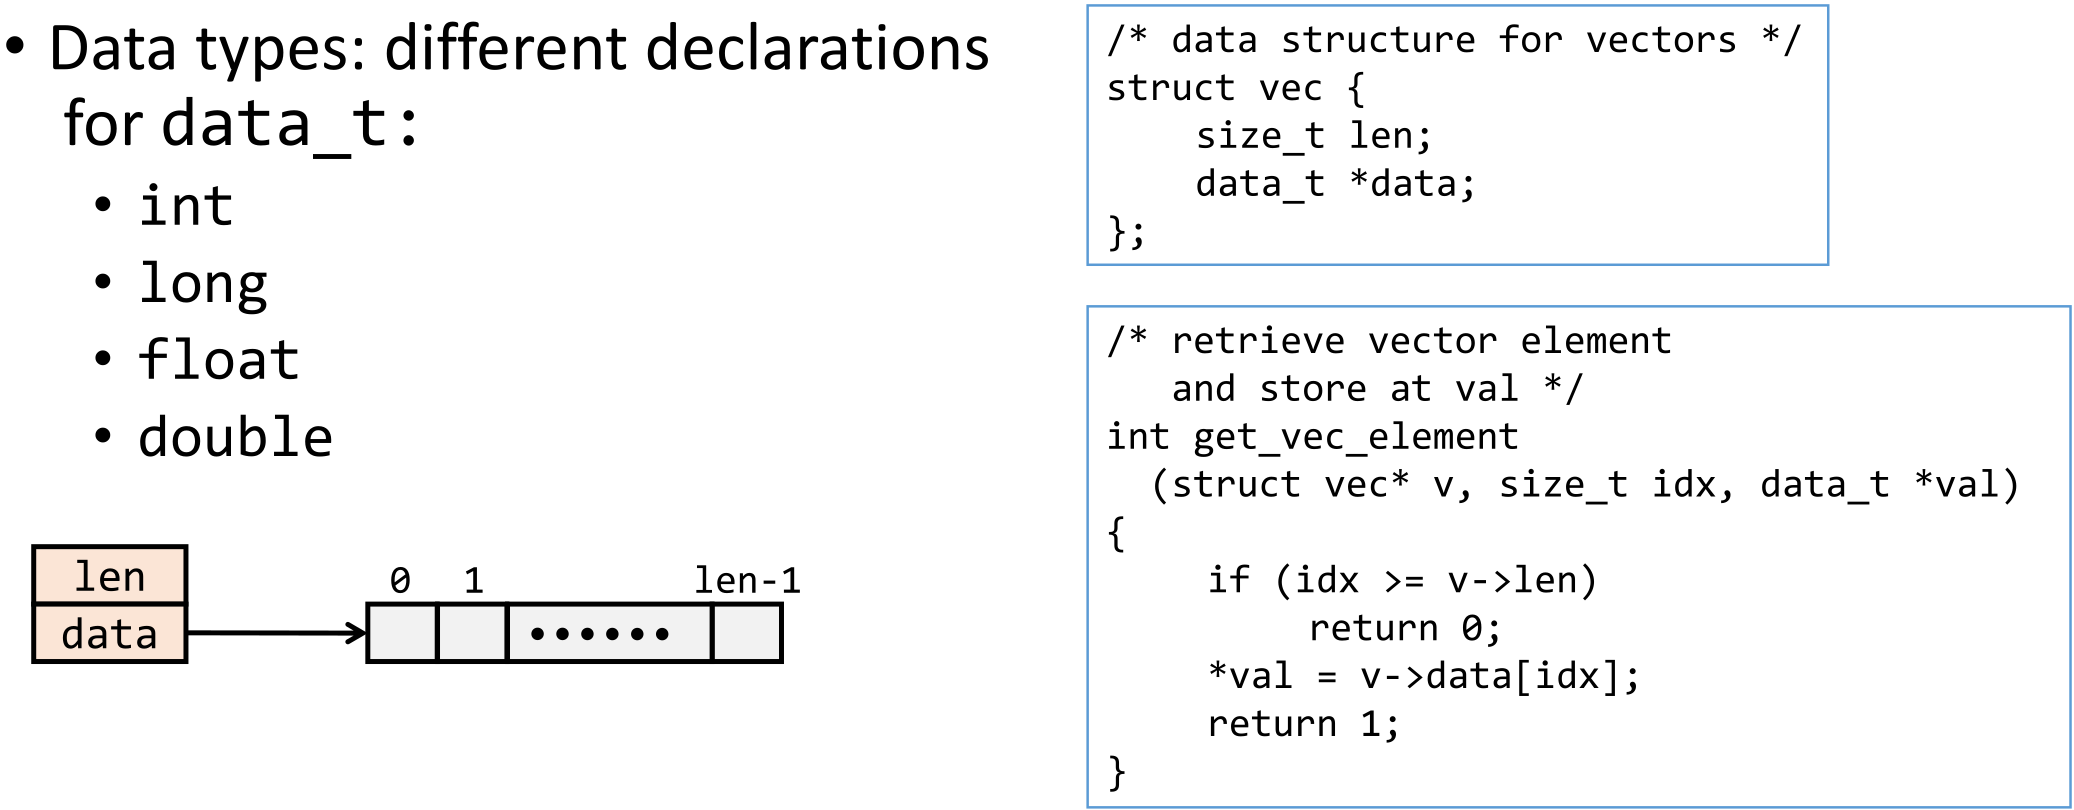
\includegraphics[width=0.8\textwidth]{17_BenchmarkStruct.png}

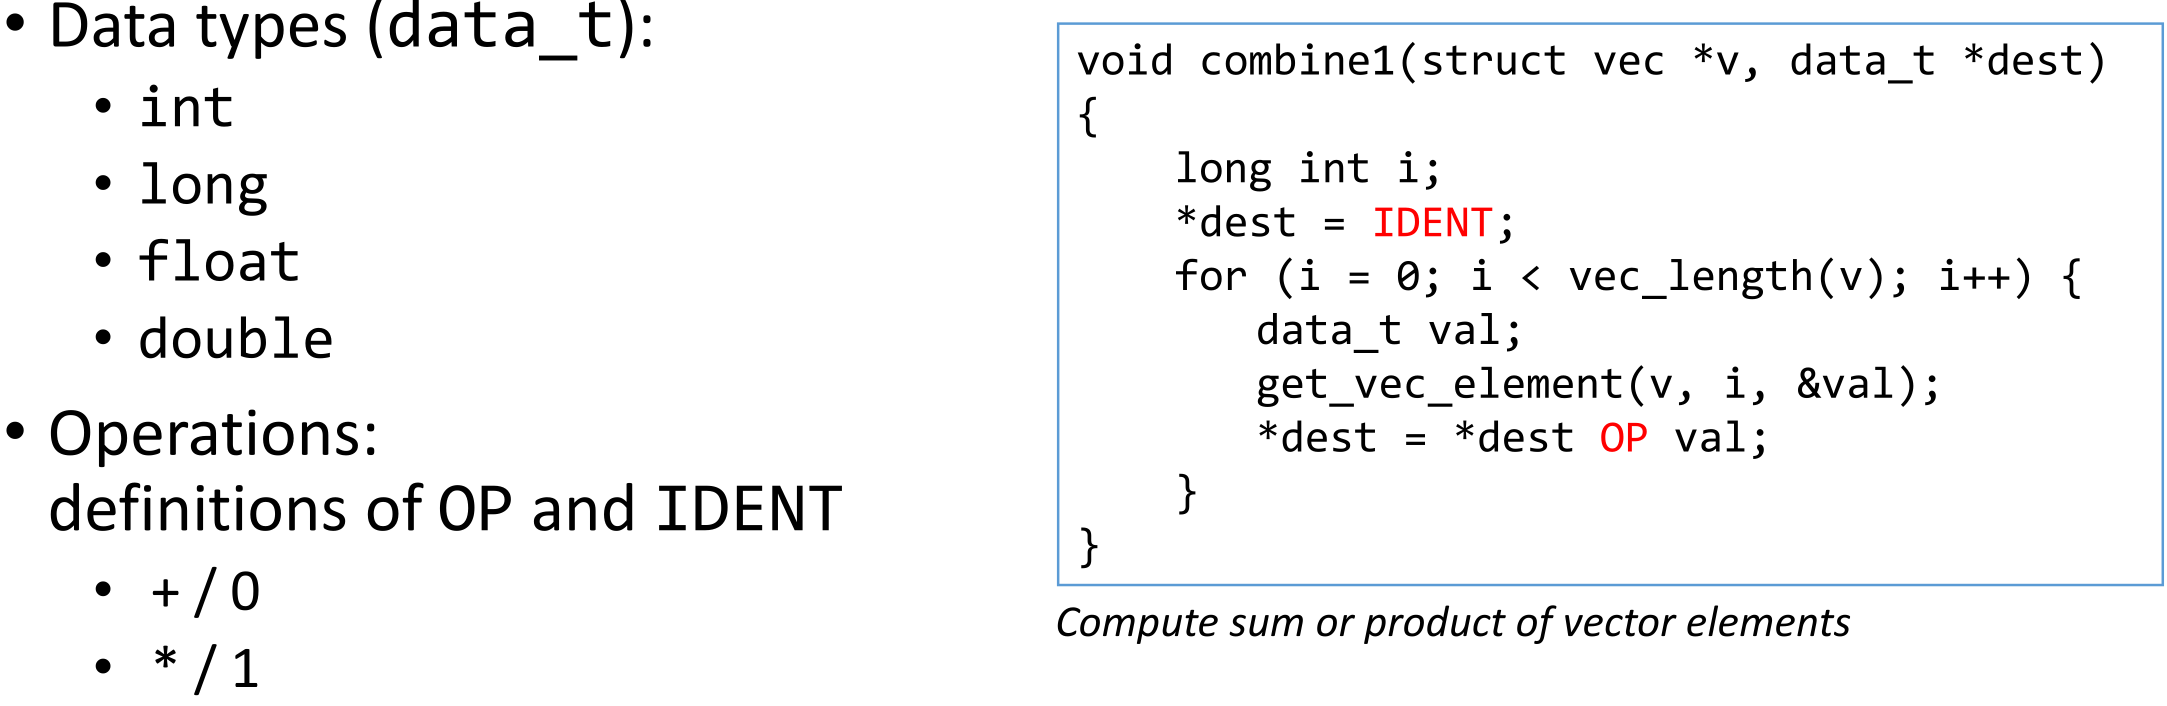
\includegraphics[width=0.8\textwidth]{17_BenchmarkCompute.png}

In order to compare different optimisations, we we need a comparable unit. The most obvious one is execution time, which is calculated as $= \text{CPE} \cdot n + \text{overhead}$. Where \textit{Cycles per Element (CPE)} is a way to express performance of a program which operates on vectors or lists.

\paragraph{Example: Base Performance}
We measure the following when running our program directly and with the \code{-01} optimizer:

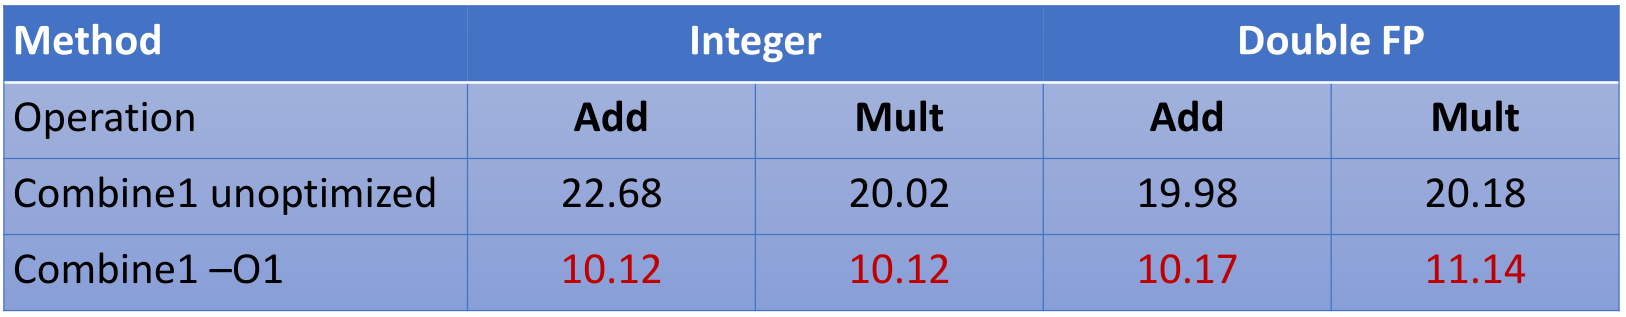
\includegraphics[width=0.8\textwidth]{17_ex1base.png}

All in all, we can observe that the optimizer shortened the execution time by a factor of two.

Some obvious optimisations we can to to our benchmark loop is:
\begin{itemize}
    \item Do \code{vec\_length} check outside of the loop.
    \item Access vector directly instead of using wrapper function \code{get\_vec\_element}.
    \item Accumulate results and write to memory after the loop.
\end{itemize}

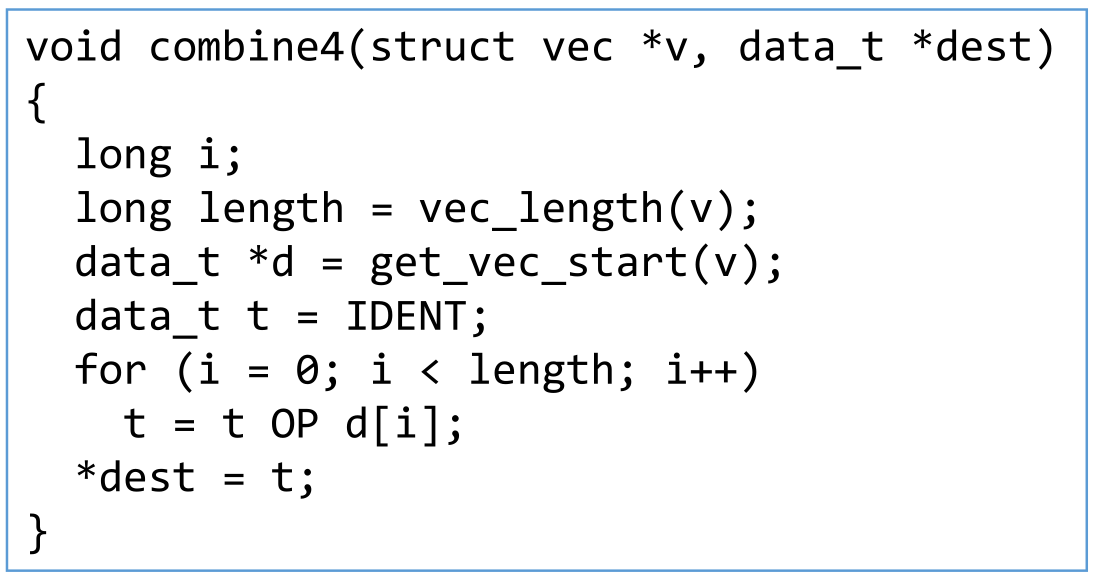
\includegraphics[width=0.8\textwidth]{17_BenchmarkComputeBasicOpt.png}

This already gives great improvements:

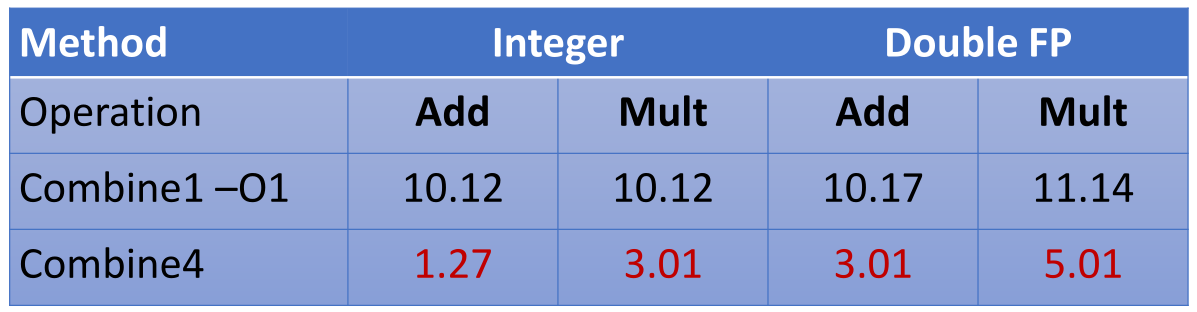
\includegraphics[width=0.8\textwidth]{17_ex1basic.png}

\subsubsection{A bit about modern processor design}

\paragraph{Sequential Processor Stages}
The fetch, decode, execute, memory, write back and pc stages are run in sequential. Since signals must propagate through instruction memory, register file, ALU and data memory in one cycle, the clock is very slow. Further hardware units are only active for a fraction of a cycle.

\paragraph{Pipelined Hardware}
The fetch, decode, execute and write-back stages are pipelined. While this allows for better utilisation of the hardware, it yields numerous problems. Most notably are data and control hazards.

\paragraph{Performance}
The program execution time is $= \text{IC} \cdot \text{CPI} \cdot CCT$
\begin{description}
    \item[IC:] Instruction count
        \begin{itemize}
            \item Increased by optimising program
        \end{itemize}
    \item[CPI:] Cycles per instruction ($= 1/\text{IPC}$)
    \item[CCT:] Clock cycle time ($=1/\text{Frequency}$)
        \begin{itemize}
            \item Increased by increasing pipeline depth
        \end{itemize}
\end{description}

 While increasing the pipeline depth leads to higher CCT, the limits are:
 \begin{itemize}
     \item Delay of pipeline registers
     \item Inequalities in work per stage since we cannot break work into stages at arbitrary points
     \item Clock skew
 \end{itemize}

The Cycles per instruction (CPI) is calculated as $=\text{CPI}_{\text{base}} + \text{CPI}_{\text{stalls}}$, where the stalls CPI is determined by the stalls due to data and control hazards, as well as due to memory latency of larger memories.

\paragraph{Superscalar Processor}
A superscalar processor can issue and execute multiple instructions in one cycle. The instructions are retrieved from a sequential instruction stream and are usually scheduled dynamically.

So a clear benefit is that is happens without programming effort. The processors can take advantage of the instruction level parallelism that most programs have.

In todays CPUs this is something very common.

The following graphics depicts the key design points

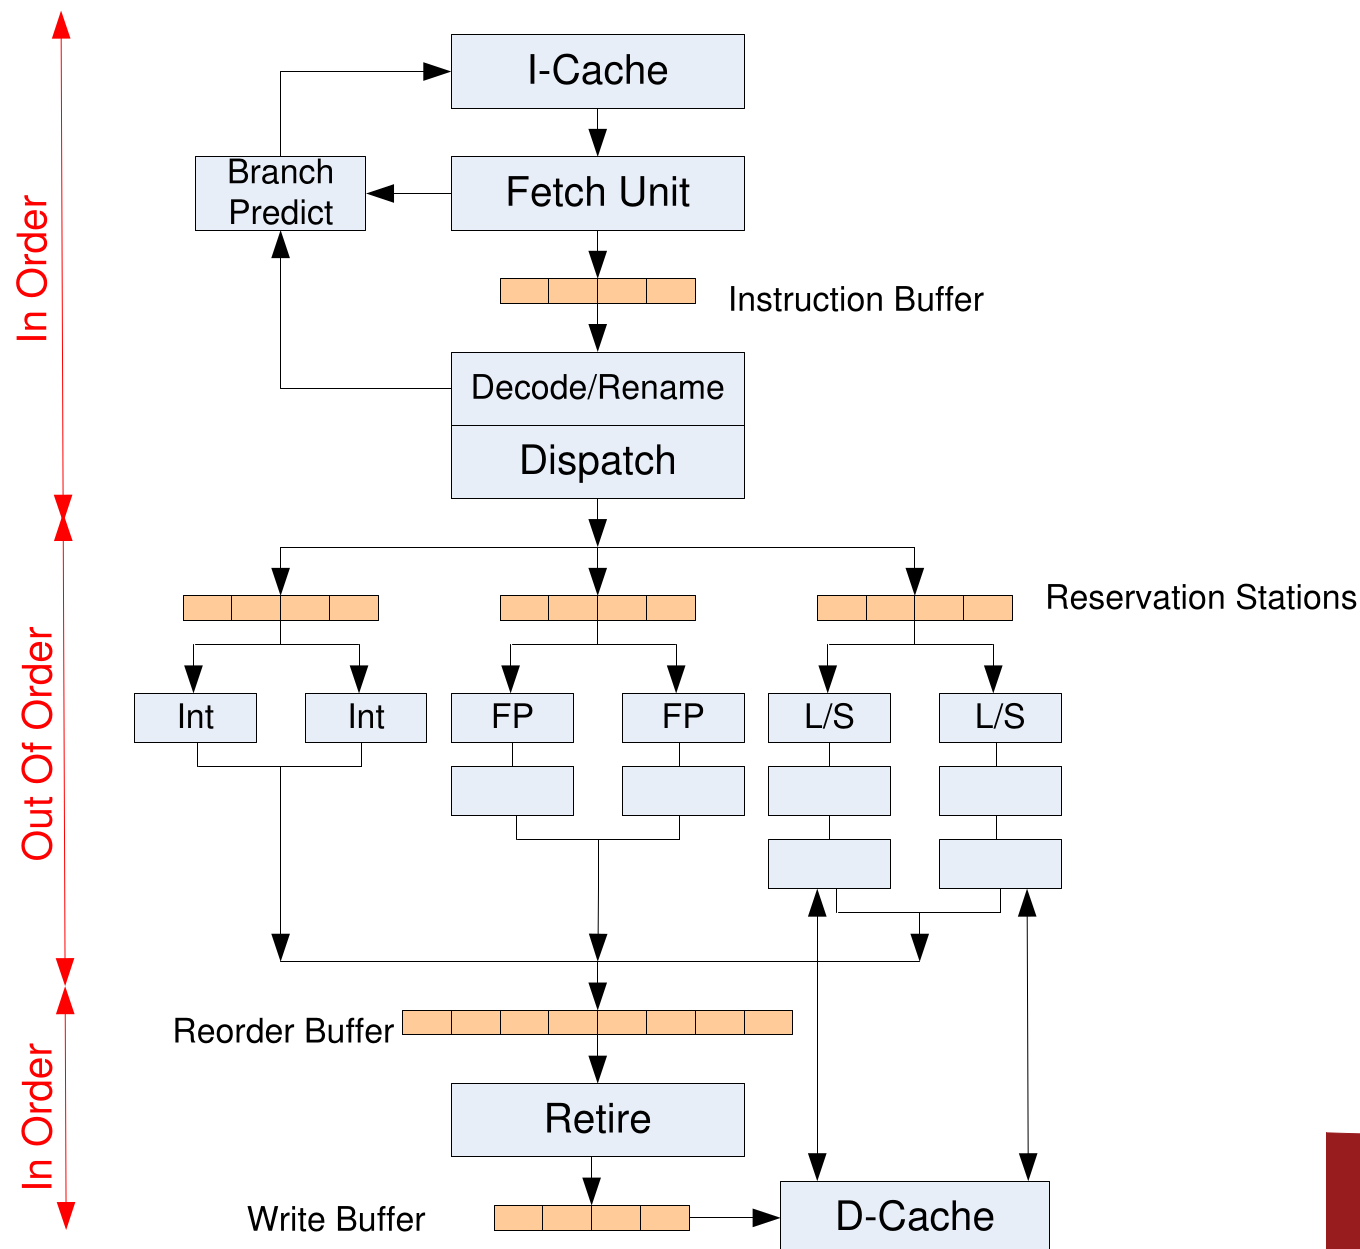
\includegraphics[width=0.8\textwidth]{17_superscalarCpuDesign.png}

\subsubsection{Superscala Processor Performance}
We analyze the performance of a super scalar processor an hand of the Intel Haswell CPU
\begin{itemize}
    \item 8 functional units
    \item Multiple instruction can execute in parallel
        \begin{itemize}
            \item 2 load + address computation
            \item 1 store + address computation
            \item 4 integer
            \item 2 FP multiply
            \item 1 FP add
            \item 1 FP divide
        \end{itemize}
\end{itemize}

The following table depicts the latency (number of cycles required) and cycles/issue (how many cycles we have to wait before issueing the next instruction in this functional unit)

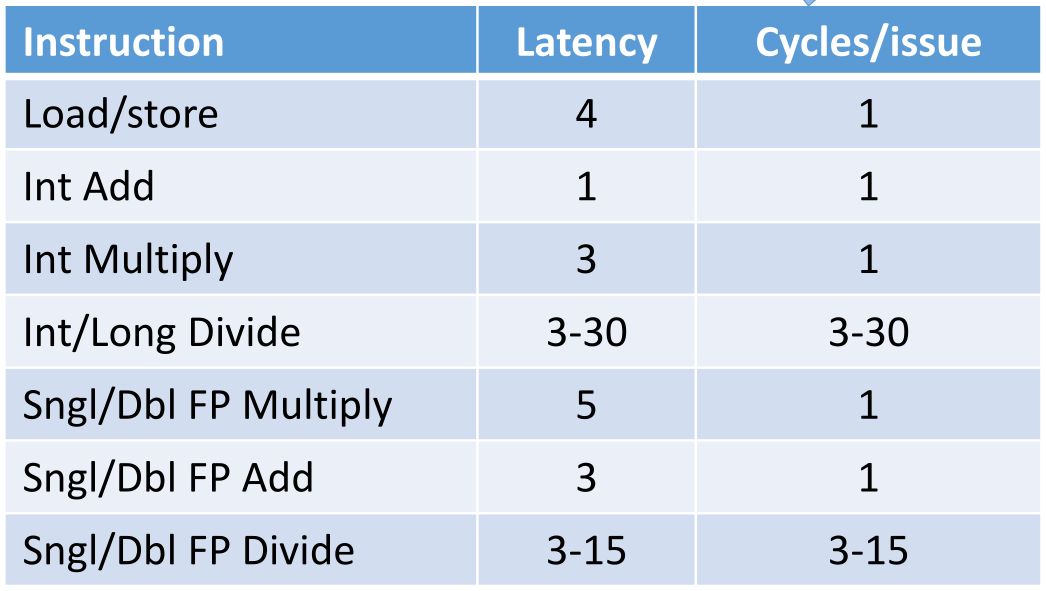
\includegraphics[width=0.8\textwidth]{17Haswell.png}

\paragraph{Latency vs Throughput}
For example FP multiplication has a latency of $5$ and cycles/issue of $1$. The execution of $5$ independent multiplications takes thus $9$ cycles to complete. In comparison, the execution of $5$ dependant instructions takes $25$ cyces to complete.

\paragraph{Data hazards}
There are three types of data hazards

\begin{description}
    \item[Read after Write (RAW):]  Only true dependency, we actually need to wait
    \item[Write after Write (WAW):] Can be fixed with  register renaming
    \item[Write after Read (WAR):] Can be fixed with register renaming
\end{description}

In register renaming we map architectural registers to a larger pool of physical registers.

\paragraph{View of Instruction Execution}
\subparagraph{Imperative View}
Imperatively, registers are viewed as fixed storage locations which are read and written to by individual instructions. Instructions are executed in a specific order to guarantee proper behaviour.

Given the following code:

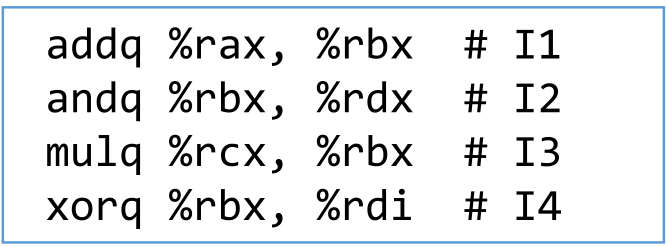
\includegraphics[width=0.8\textwidth]{17_exInstuctionExecutionCode.png}

The imperative view looks als follows:

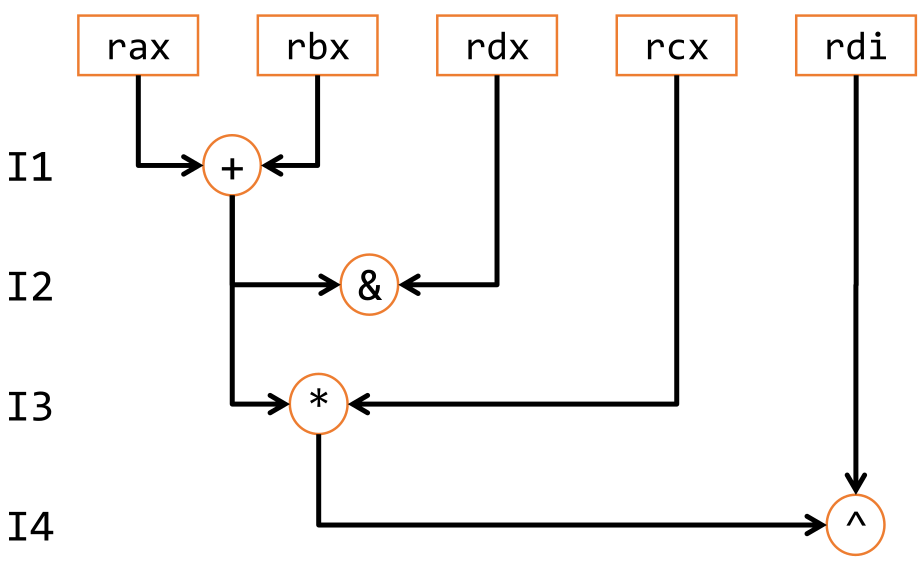
\includegraphics[width=0.8\textwidth]{17_exInstuctionExecutionImp.png}

\subparagraph{Functional View}
From a functional perspective we can view the execution of instruction as a dependency graph. Each write as creating new insurances of a value. So, operations can perform as soon as all operands are available. The sequence of execution may differ from the original instruction sequence.

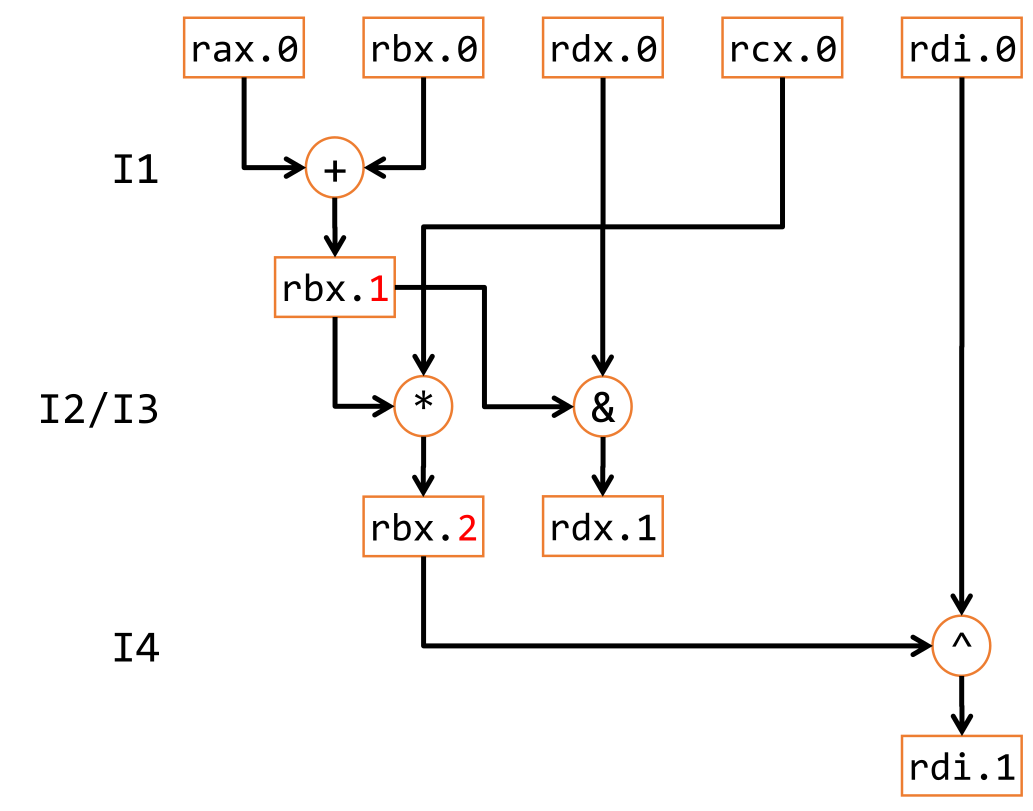
\includegraphics[width=0.8\textwidth]{17_exInstructionExecutionFunc.png}

\paragraph{Performance Bounds}
There are two types of bounds.
\subparagraph{Latency Bound}
The latency bound limits the performance, when operations must be executed sequentially. Therefore, the latency bound is simply the latency of the functional unit.

The performance is determined by the latency of the operation. So, the latency bound of our benchmark problem is simply the latency of the designated operation. For a vector of length $8$ and multiplication operation, we get following \textit{dependency graph}:

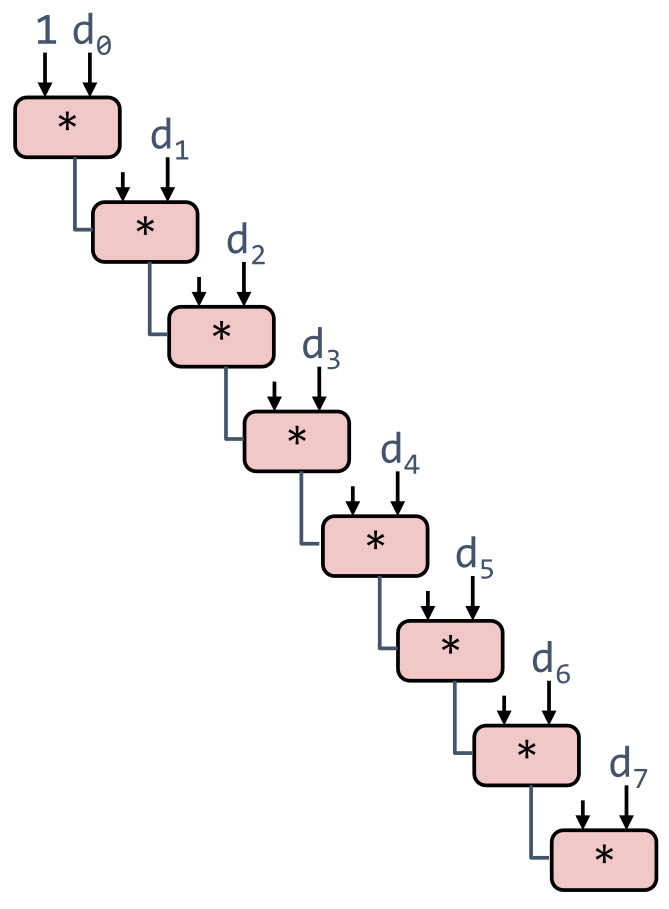
\includegraphics[width=0.8\textwidth]{17_serialcomputation.png}

For the Intel Haswell example, we get

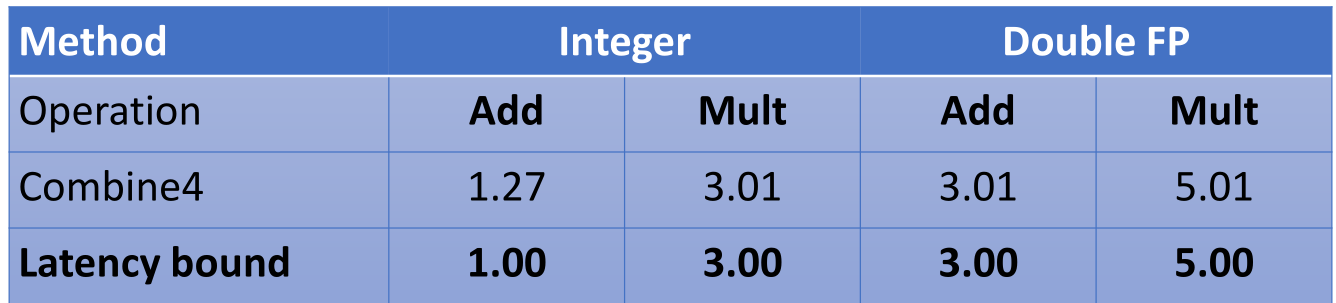
\includegraphics[width=0.8\textwidth]{17_latencyBoundIntel.png}

\subparagraph{Loop Unrolling ($2x1$)}
Loop unrolling in the action of repeat a loop fewer times, but do more computation in one execution. For example a $2x1$ unrolling does $\frac{1}{2}$ as many iteration but $2x$ as much work per iteration.

Our benchmark code

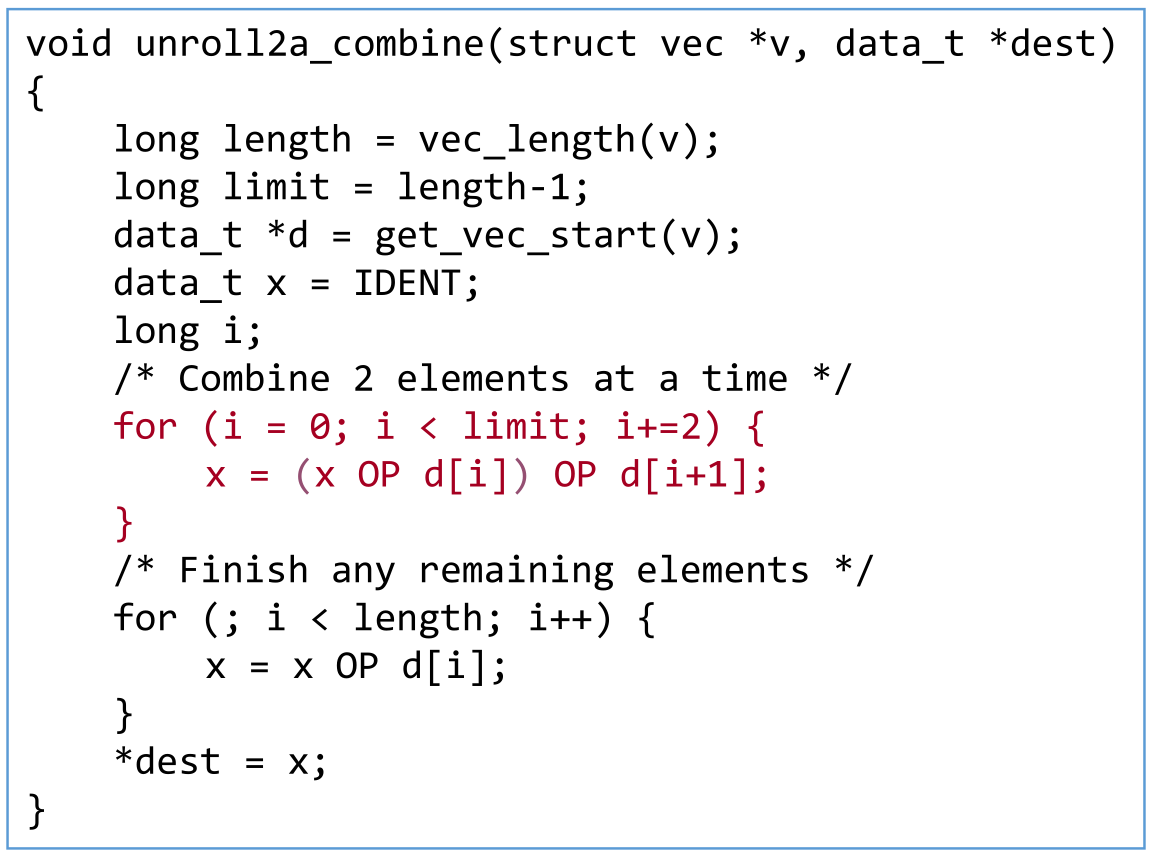
\includegraphics[width=0.8\textwidth]{17_loopunrollingcode.png}

We get a performance of 

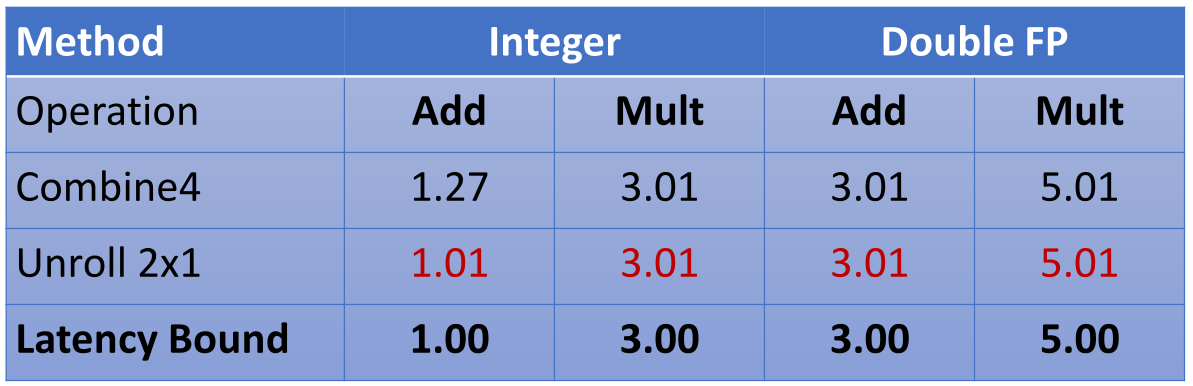
\includegraphics[width=0.8\textwidth]{17_loopunrollingperformance.png}

We can see that only the performance of the integer addition has improved. All other operation stay the same, because they are still sequentially dependant.


\subparagraph{Throughput Bound}
The throughput bound is the bound of the performance when instructions can execute in parallel.

Throughput for no parallel execution is calculated as $1 / \text{cycles/issue}$. When multiple instructions are run in parallel, the formula is $\text{throughputSeq} / \text{\#parallelInstruction}$. To get the throughput bound, we have to take the maximum of the throughput of the operation itself and the throughput of the load/store operation. This is because the load/store operation may be the bottleneck.

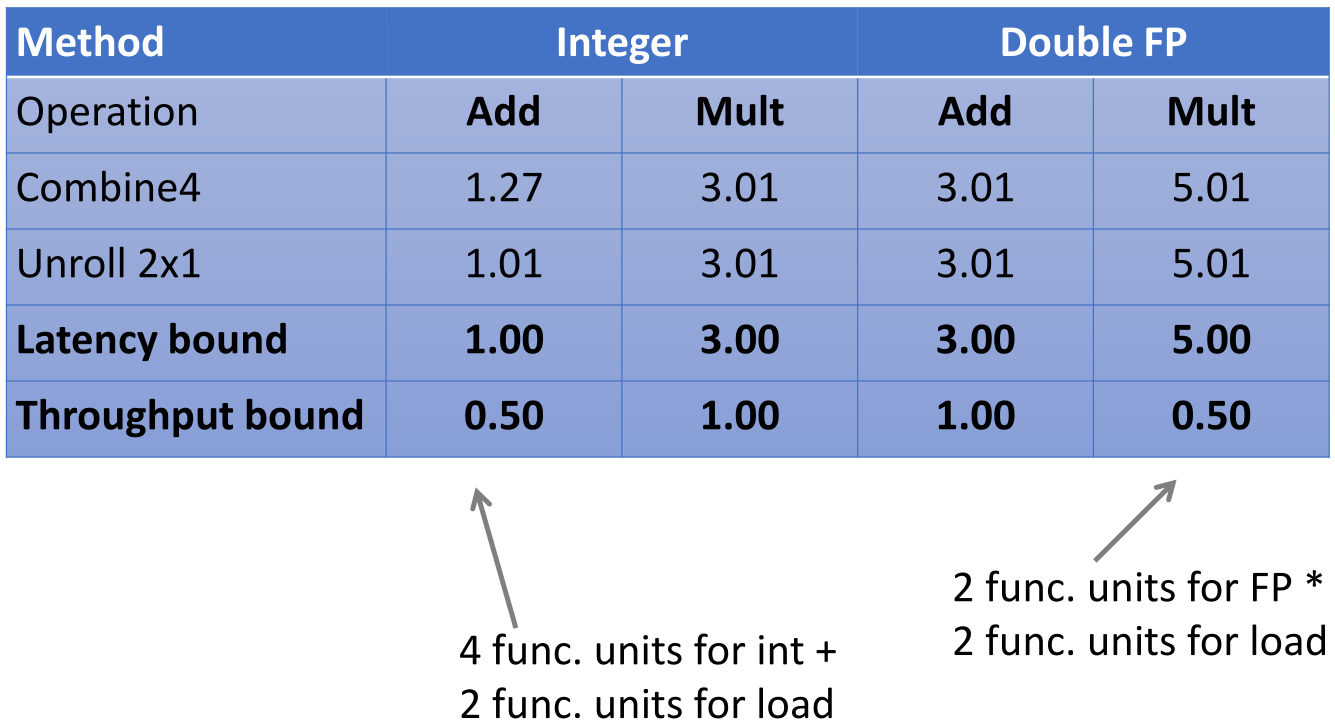
\includegraphics[width=0.8\textwidth]{17_performanceBoundTable.png}

\subsubsection{Reassociation}
The idea of reassociation is to change the order of the brackets in order to create an independant operation. So it can be scheduled in parallel. In the previous loop unrolling the changed to computation to $x = (x \text{ OP } d[i]) \text{ OP } d[i + 1]$. Now the change it to $x = x \text{ OP } (d[i] \text{ OP } d[i + 1]$.

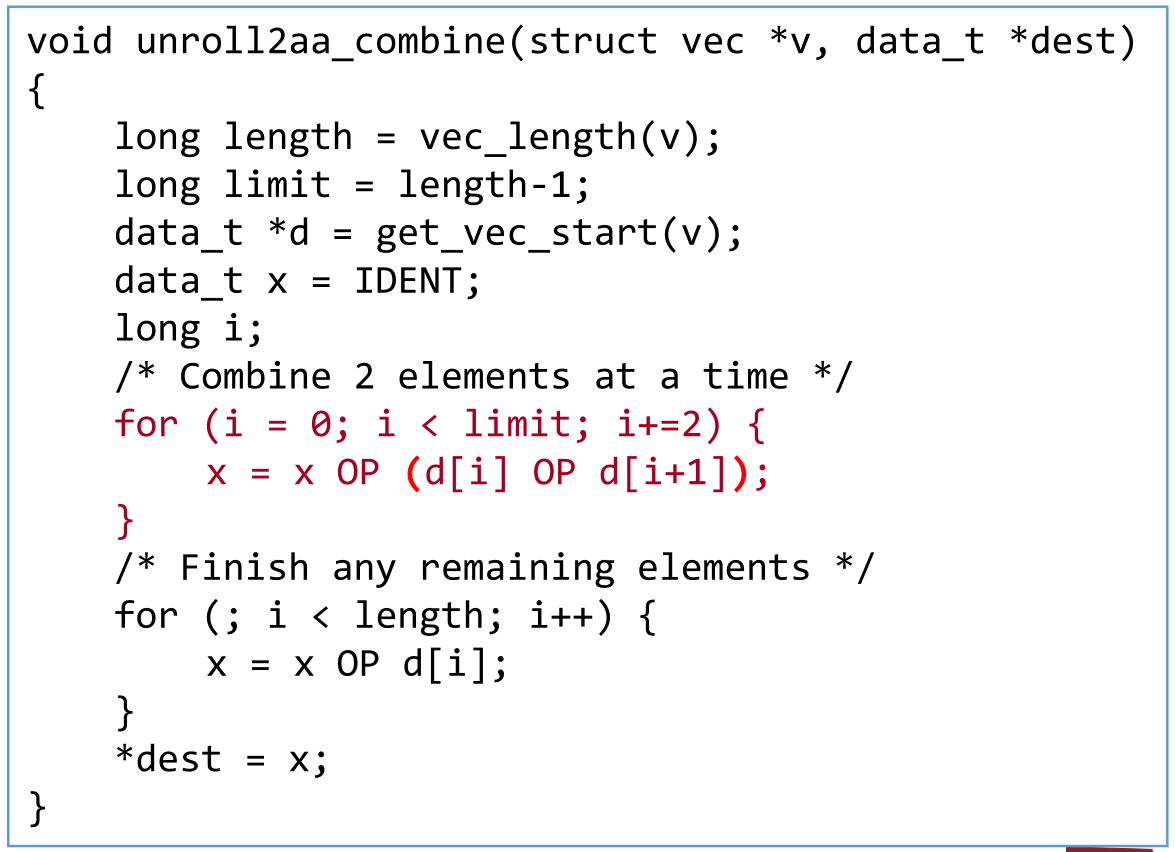
\includegraphics[width=0.8\textwidth]{17_reassociationunrollingcode.png}

The graph for the multiplication of $8$ elements looks as

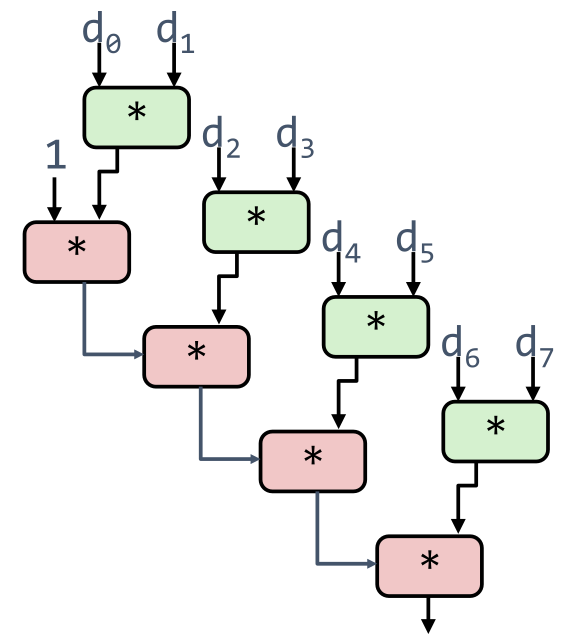
\includegraphics[width=0.8\textwidth]{17_reassocatedcomputationgraph.png}


But one has to notice, that for FP this may change the results, since FP operations are not associative.

For our benchmark we get a nearly $2x$ speedup for FP addition and FP and integer multiplication. This is due to the sequential dependency.

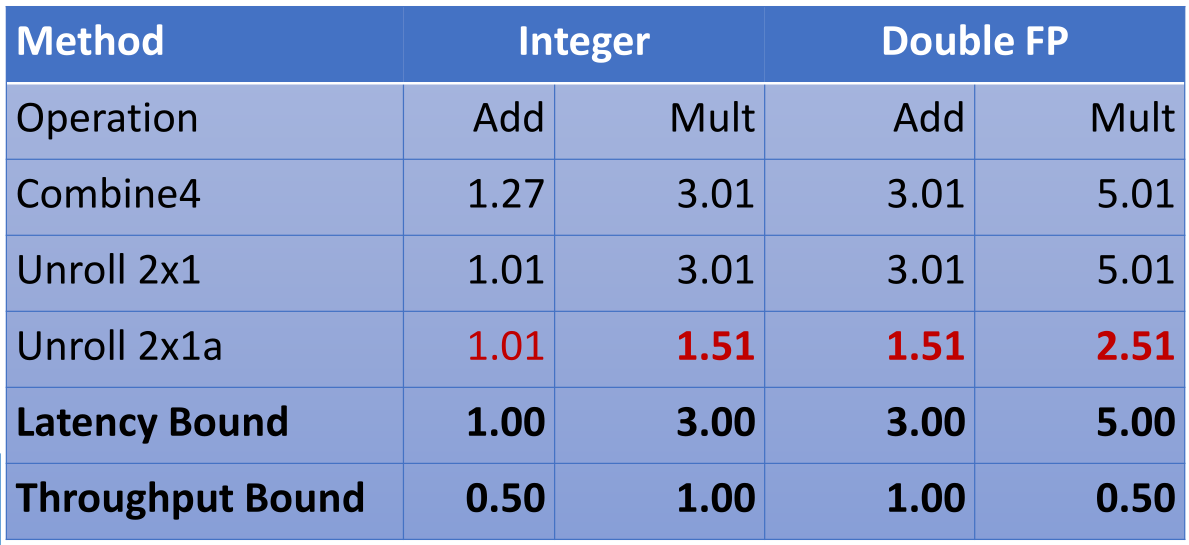
\includegraphics[width=0.8\textwidth]{17_reassocationunrollingtable.png}

\subparagraph{Loop Unrolling with Separate Accumulators ($2x2$)}
Another idea is to increase the number of accumulators. This yields a different for of reassociation.

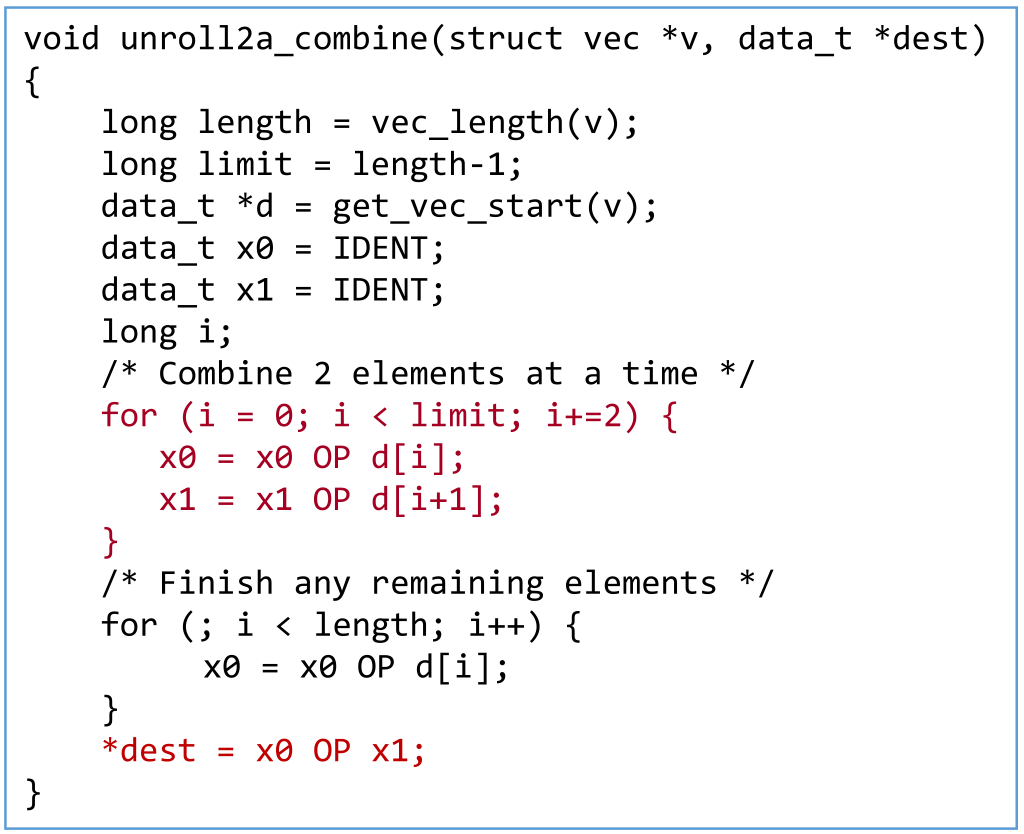
\includegraphics[width=0.8\textwidth]{17_seperateaccumulators.png}

This way we get two independant \textit{streams} of operations

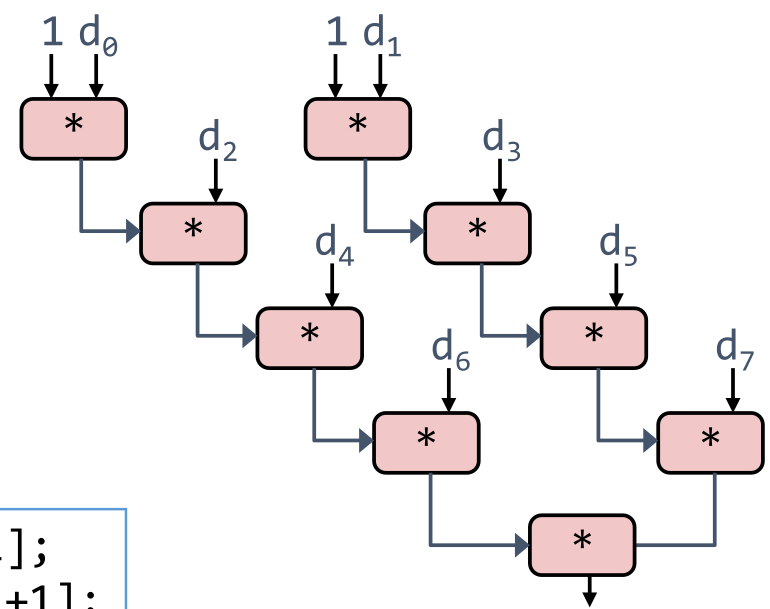
\includegraphics[width=0.8\textwidth]{17_seperateAccumulatorsGraph.png}

Concerning our benchmark performance, integer addition can make use of two load units and for integer and FP multiplication and FP addition we get a $2x$ speedup compared to the $2x1$ unrolling

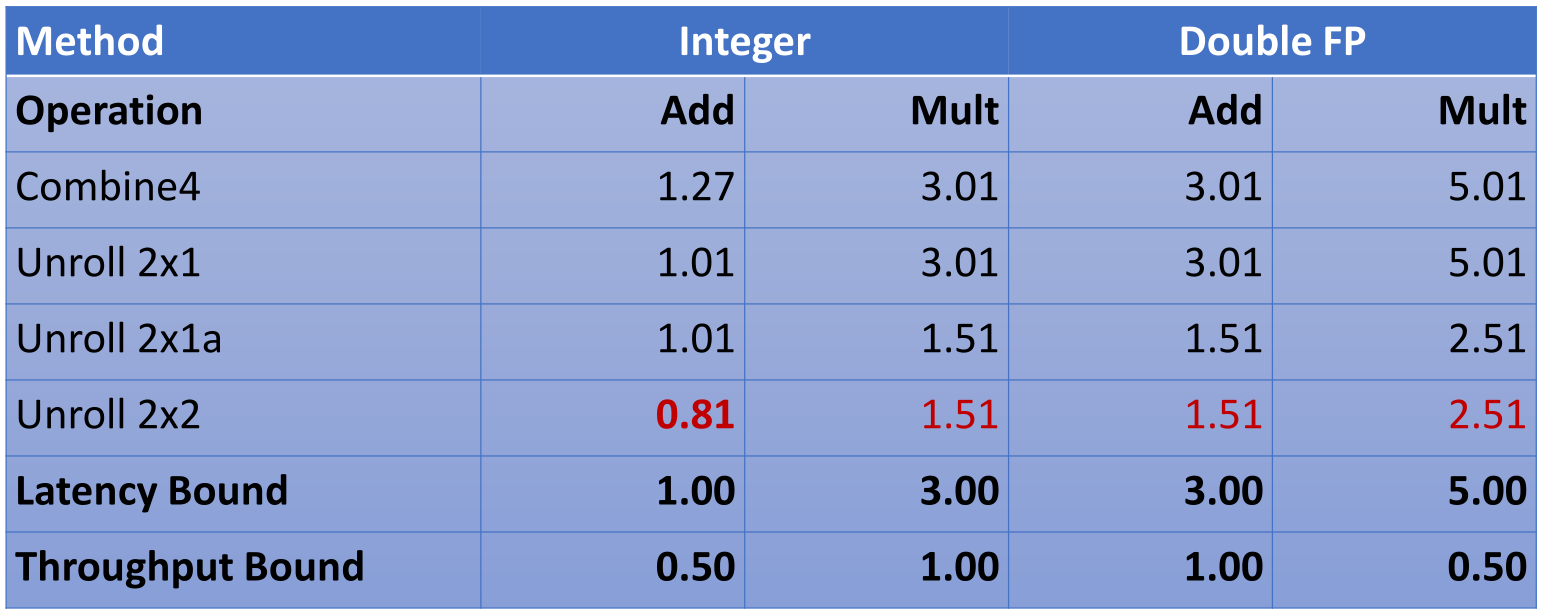
\includegraphics[width=0.8\textwidth]{17_seperateAccumulatorsTable.png}

\subsubsection{Combining Multiple Accumulators and Unrolling}
The idea is to unroll the loop to a degree of $L$ and accumulate $K$ results in parallel ($L$ must be a multiple of $K$). The limitations for this are diminishing returns since we cannot go beyond throughput limitations, and we also get large overheads for short lengths.

The best values can only be evaluated through tests. Compiler cannot do these kind of improvements.

\paragraph{Double Multiplication}
For double multiplication on Intel Haswell we get

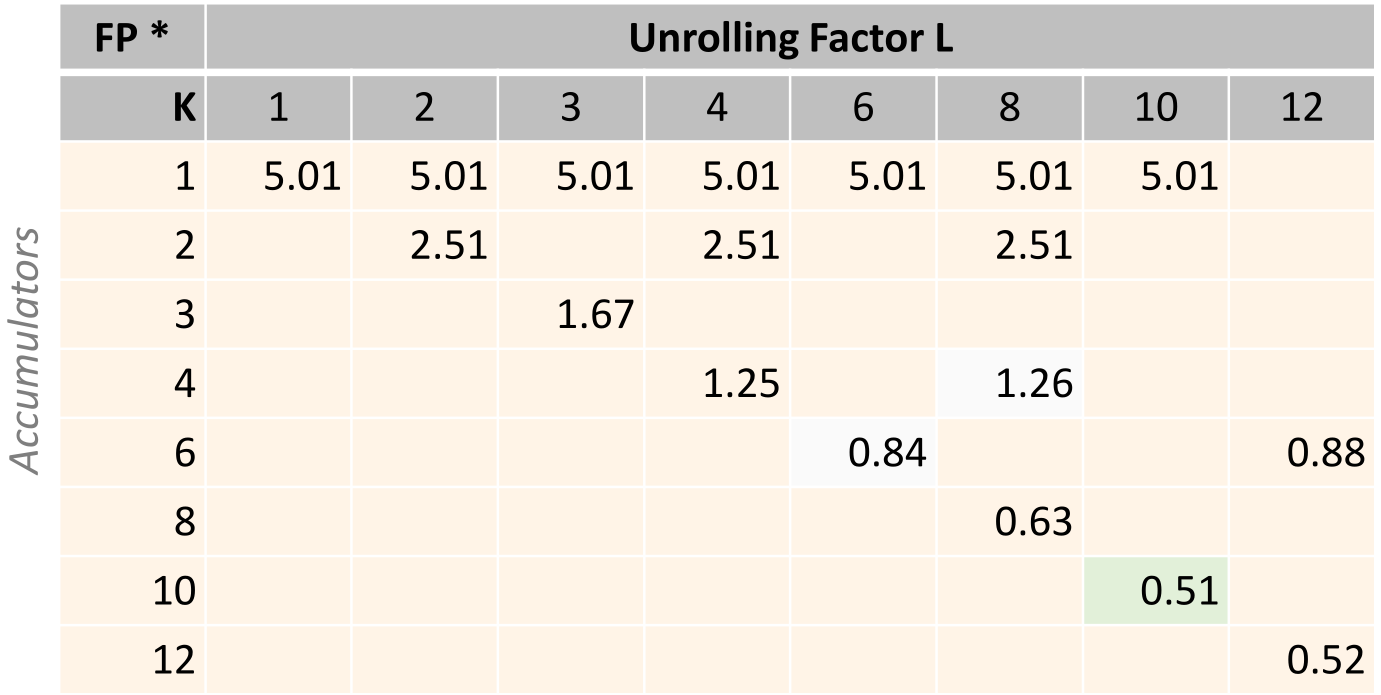
\includegraphics[width=0.8\textwidth]{17_rollandaccumdoublemult.png}

\paragraph{Integer Addition}
For integer addition on Intel Haswell we get

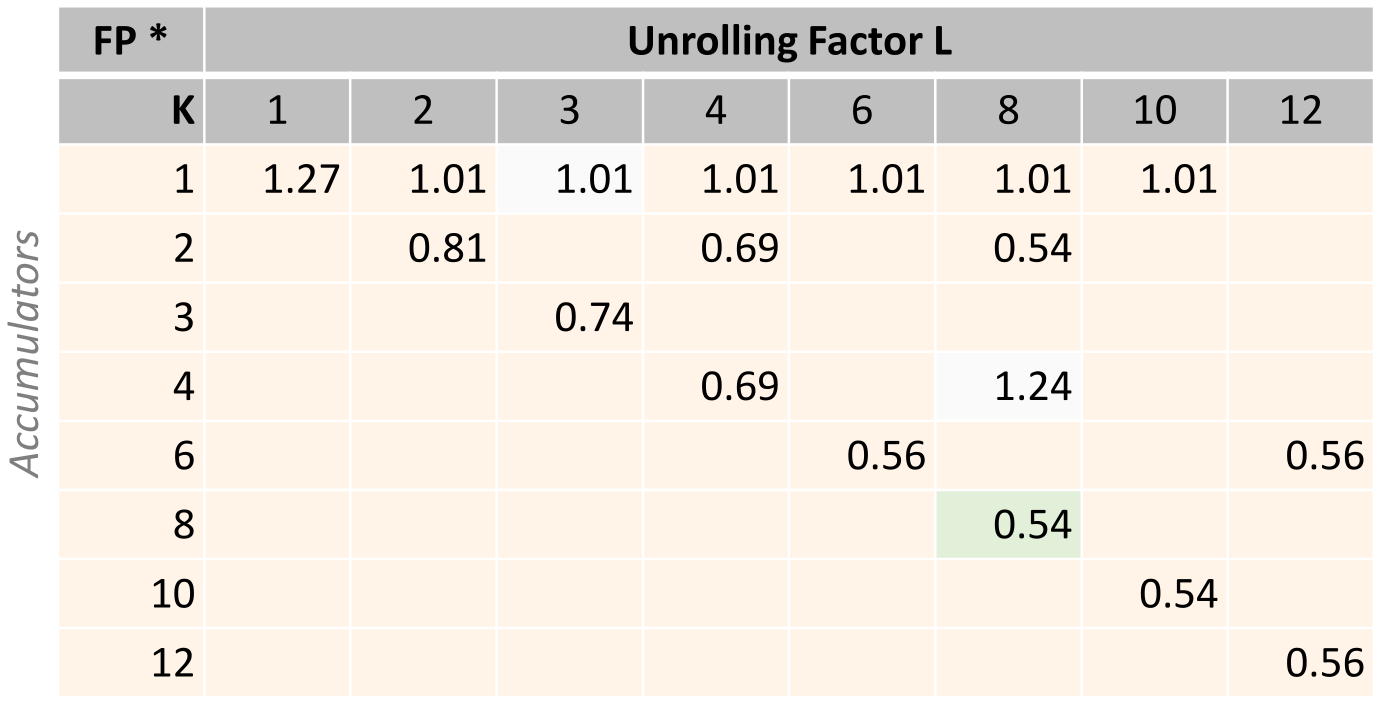
\includegraphics[width=0.8\textwidth]{17_rollandaccumintegeradd.png}

\paragraph{Summary}
Using the described methods the best performance we could achieve are

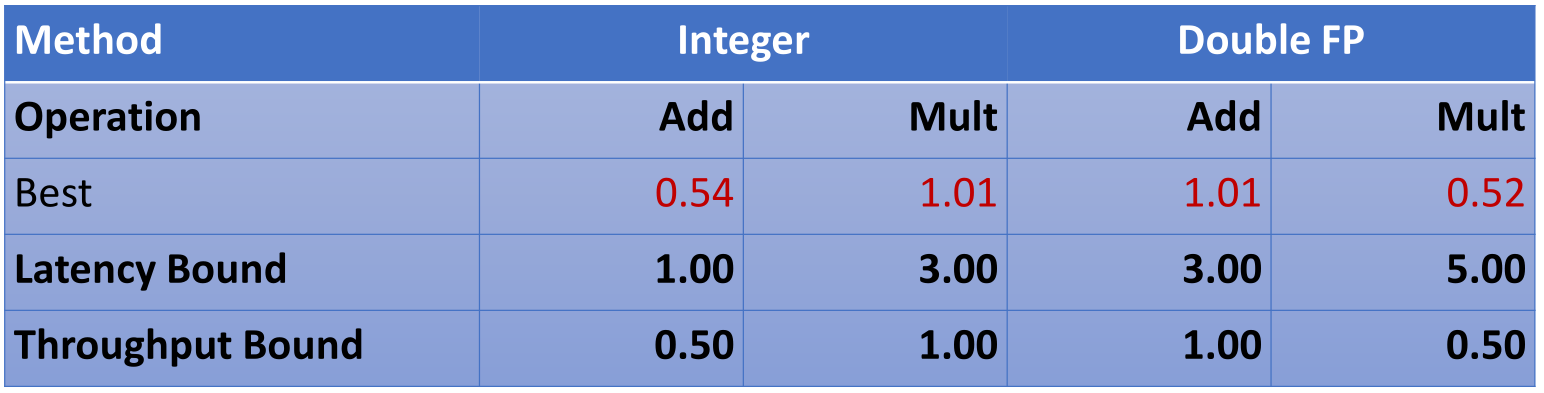
\includegraphics[width=0.8\textwidth]{17_bestperformance.png}

It is limited only be the throughput of the functional units.

\paragraph{SIMD}
The only way to do even better is using SIMD instructions. Using the AVX2 SIMD operations on $256$-bit vectors yields

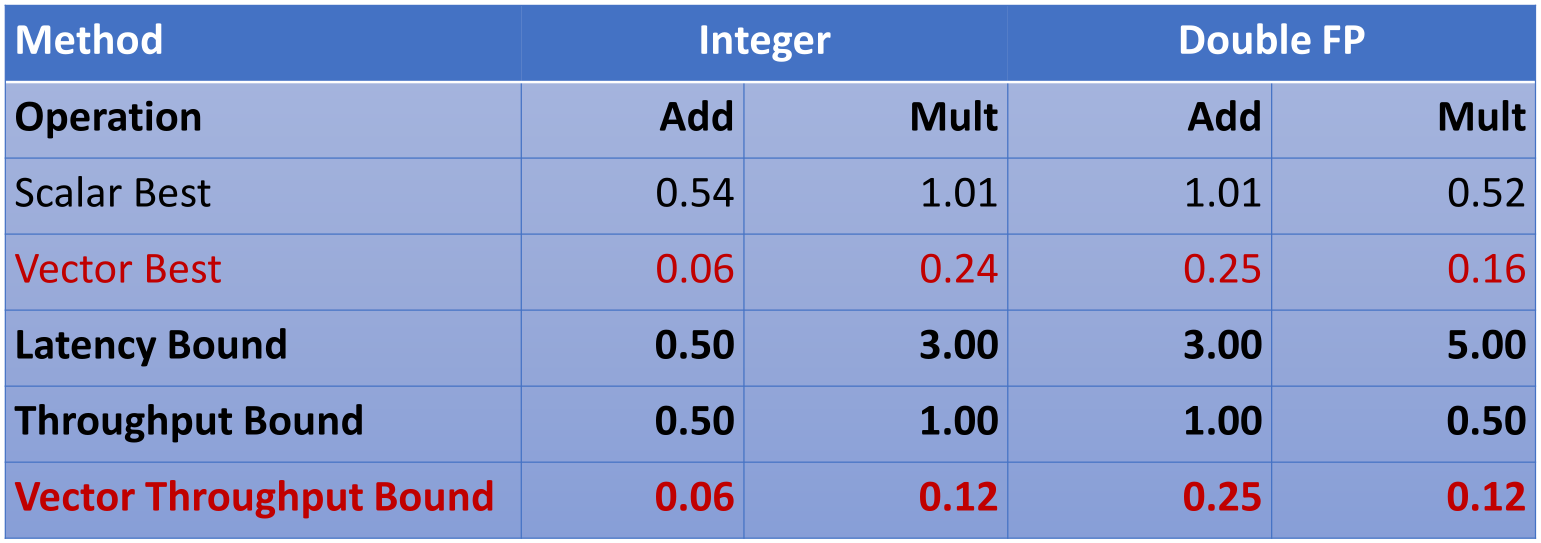
\includegraphics[width=0.8\textwidth]{17_simdperformance.png}
